%\cleardoublepage
%\thispagestyle{empty}
\mbox{}

\chapter{Resultados}
\label{ch:chapte5}

\section{Conjunto de datos hiperespectrales}

Para realizar los experimentos, se han utilizado diferentes conjuntos de datos hiperespectrales, tanto reales como sintéticos:

\begin{figure}
\centering
\begin{tabular}{cc}
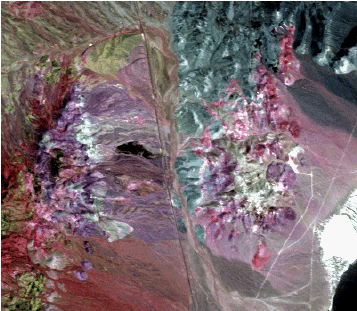
\includegraphics[height=0.35\textwidth]{images/cupritecolor.png} &
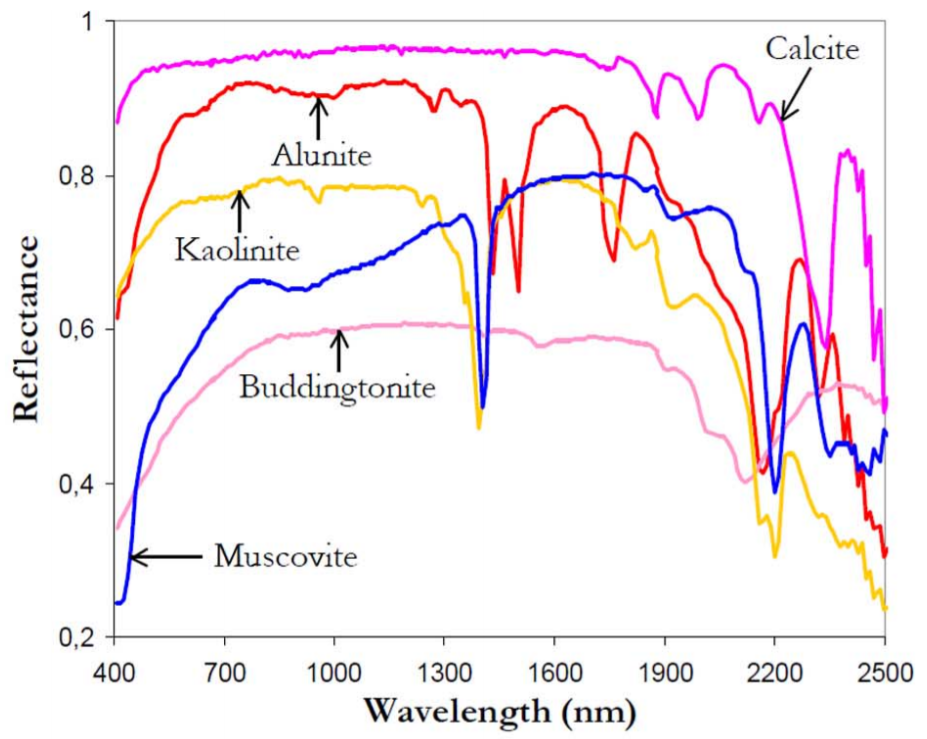
\includegraphics[height=0.35\textwidth]{images/cupriteSignatures.png}\\
(a) & (b)\\
\end{tabular}
\caption{(a) Composición en falso color de la escena captada por el sensor hiperespectral AVIRIS sobre el distrito minero de Cuprite en Nevada. (b) Firmas espectrales de la biblioteca U.S. Geological Survey de los minerales expuestos de interés.} \label{fig:aviriscuprite}
\end{figure}

\begin{itemize}
    \item El primer conjunto de datos corresponde a la conocida escena AVIRIS Cuprite (ver Figura \ref{fig:aviriscuprite}(a)), recogida en el verano de 1997 y disponible online en unidades de reflectancia después de ser corregida atmosféricamente. La porción utilizada en los experimentos corresponde a un subconjunto de 350 x 350 píxeles del sector, etiquetados como f970619t01p02\_r02\_sc03.a.rfl en los datos online, que cuenta con 224 bandas espectrales en el rango de 400 a 2500 nanómetros y un tamaño total de alrededor de 50 megabytes. Las bandas 1-3, 105-115 y 150-170 han sido eliminadas antes del análisis debido a la absorción por agua y la baja relación señal-ruido o signal-to-noise ratio (SNR) de estas bandas. La zona es bien conocida mineralógicamente, y tiene varios minerales expuestos de interés, incluyendo alunita, buddingtonita, calcita, caolinita y moscovita. Las firmas de referencia de suelo de los minerales mencionados (ver Figura \ref{fig:aviriscuprite}(b)), disponibles en la biblioteca U.S. Geological Survey library (USGS), se utilizarán para evaluar la pureza de la firma de los endmembers en este trabajo.
    
    \item El segundo conjunto de datos corresponde a una imagen sintética (ver Figura \ref{figure:synthetic}) que nos ayudará a evaluar la escalabilidad de nuestras implementaciones. La imagen ha sido construida usando un conjunto de 30 firmas espectrales de la librería USGS y el procedimiento descrito en \cite{miller1986definition} para simular patrones naturales espaciales. La imagen sintética resultante está compuesta por un total de 750$\times$650 píxeles y 224 bandas espectrales, dando como resultado un tamaño aproximado de 437 MB. La Figura \ref{figure:synthetic} muestra una composición en falso color de la escena simulada y tres ejemplos de mapas de abundancia verdad terreno (construidos a partir de píxeles puros o endmembers).
    
\end{itemize}

\begin{figure}[ht]
\centering
\begin{tabular}{cc}
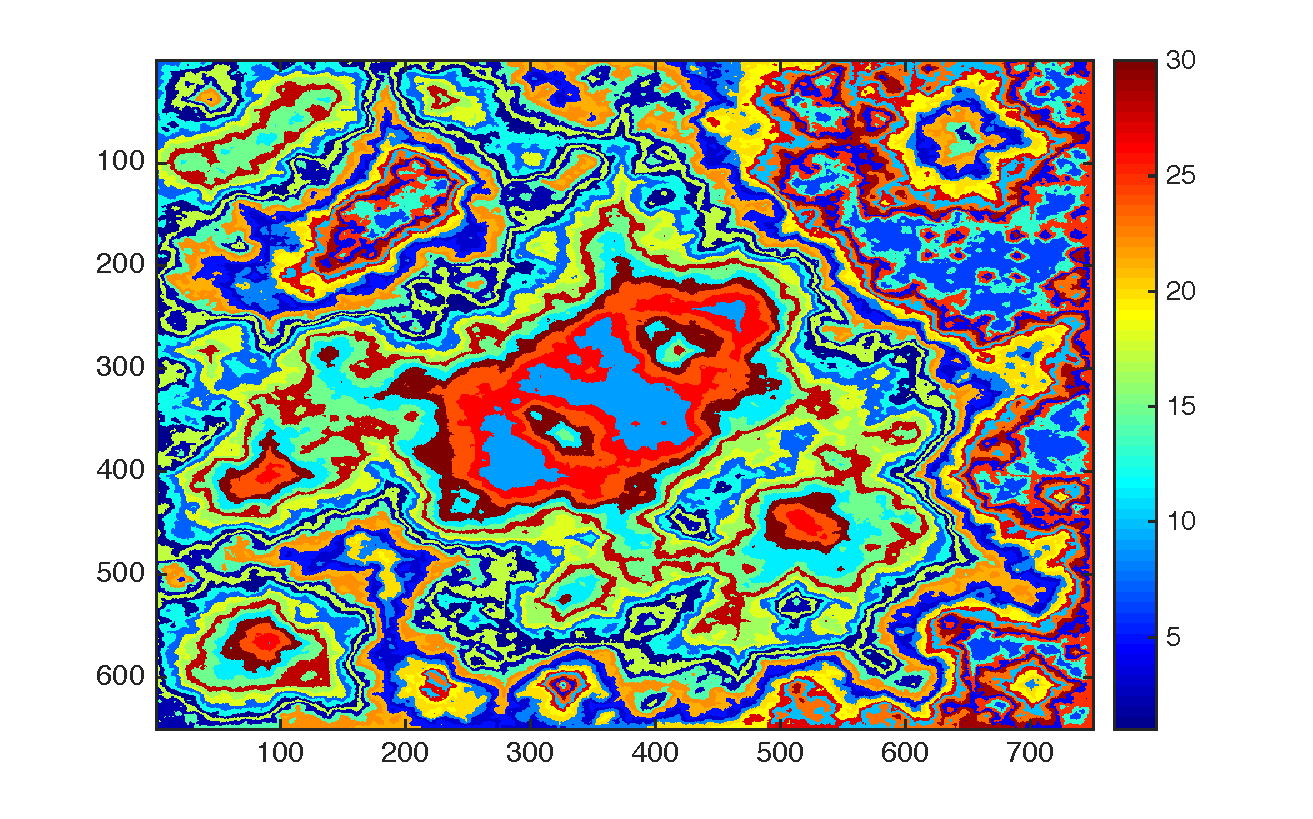
\includegraphics[height=0.30\textwidth]{./images/Synthetic1.pdf} &
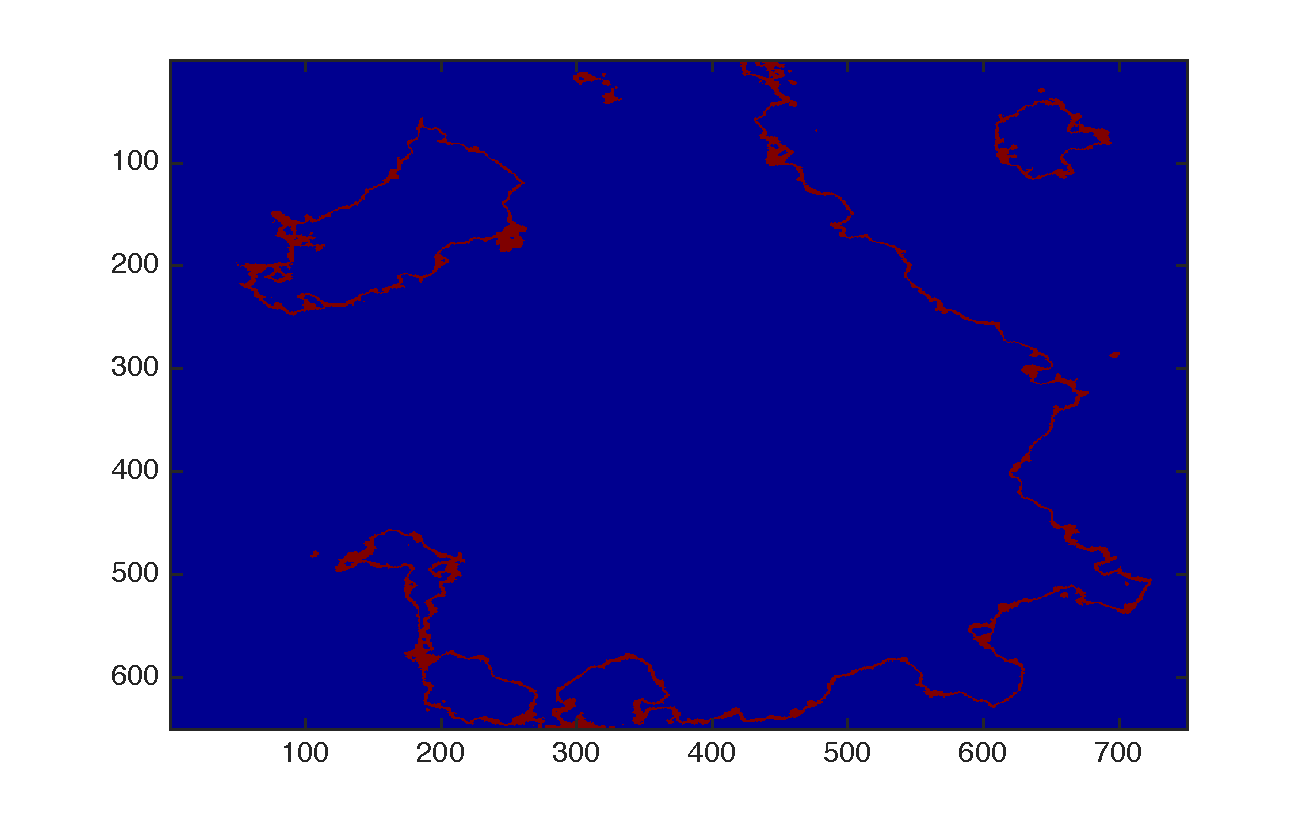
\includegraphics[height=0.30\textwidth]{./images/Synthetic1_end_3.pdf}\\
(a) & (b)\\
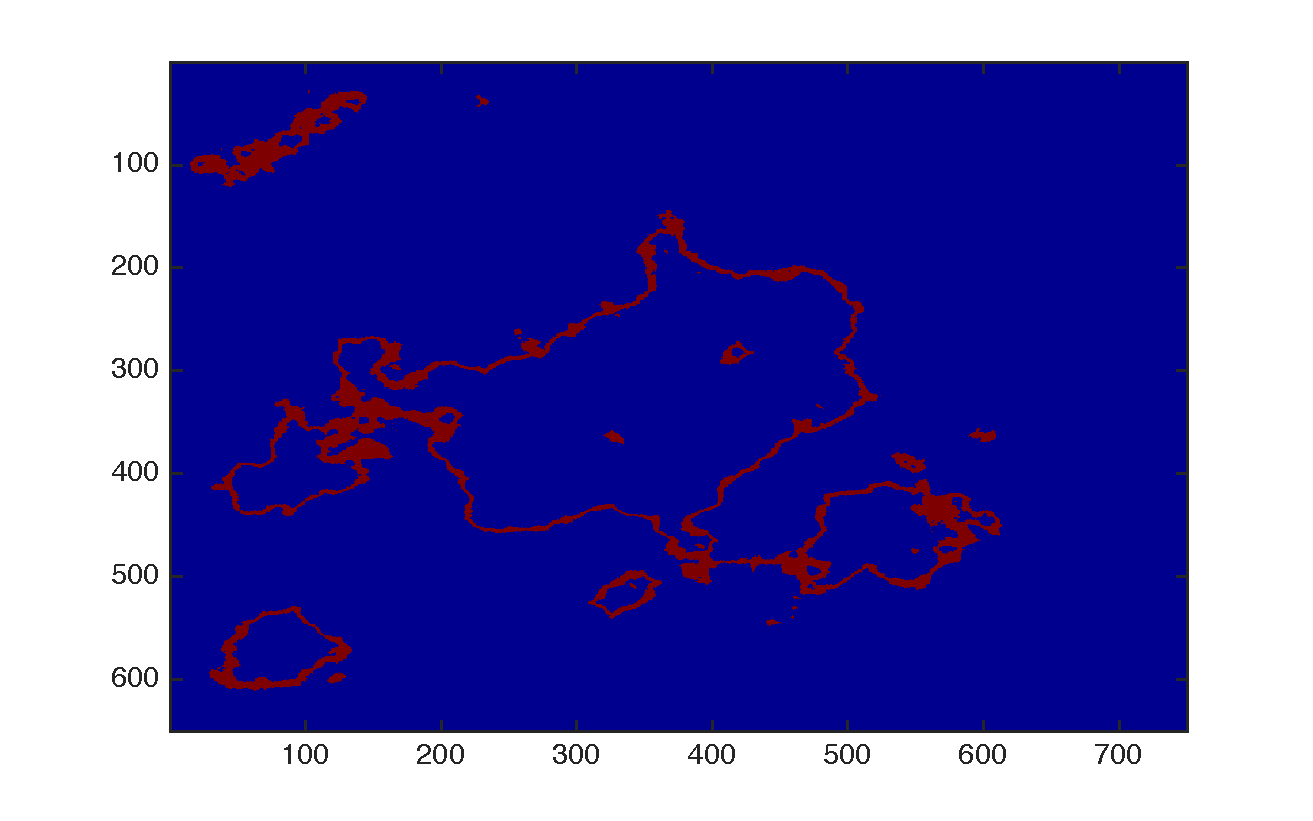
\includegraphics[height=0.30\textwidth]{./images/Synthetic1_end_15.pdf} &
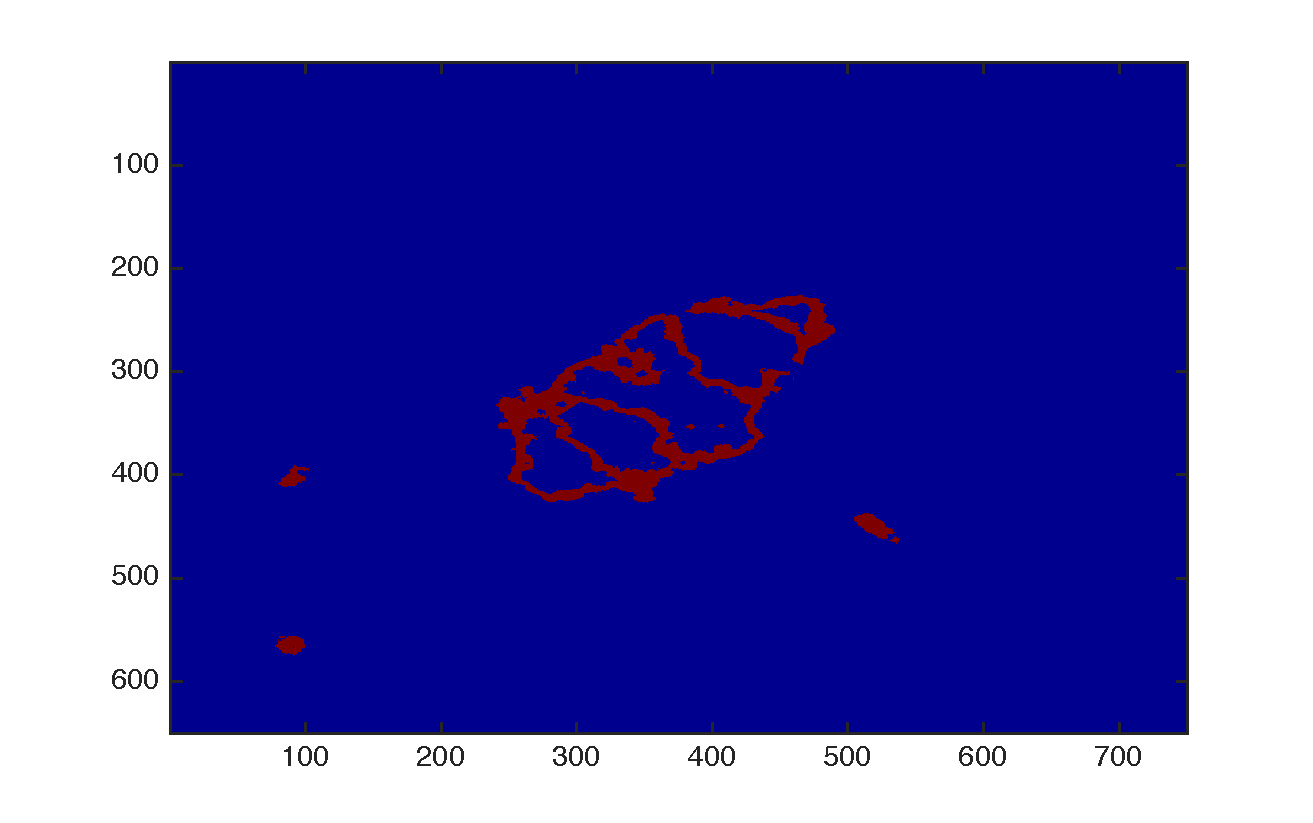
\includegraphics[height=0.30\textwidth]{./images/Synthetic1_end_26.pdf}\\
(c) & (d)\\
\end{tabular}
\caption{(a) Composición en falso color de la escena sintética. (b) Endmember \#3. (c) Endmember \#15. (d) Endmember \#26.}
\label{figure:synthetic}
\end{figure}

\section{Plataformas FPGAs}

\begin{figure}
  \centering
    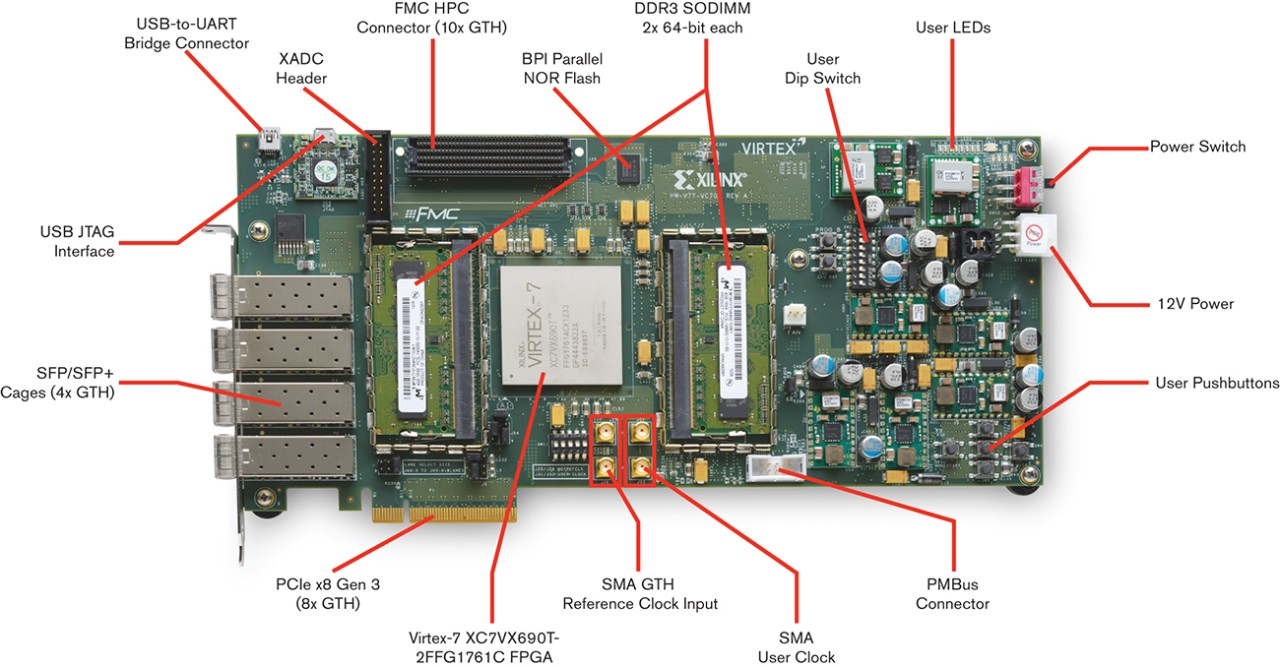
\includegraphics[width=1\textwidth]{images/VC709.png}
  \caption{Placa VC709.}
  \label{fig:VC709}
\end{figure}

\begin{figure}
  \centering
    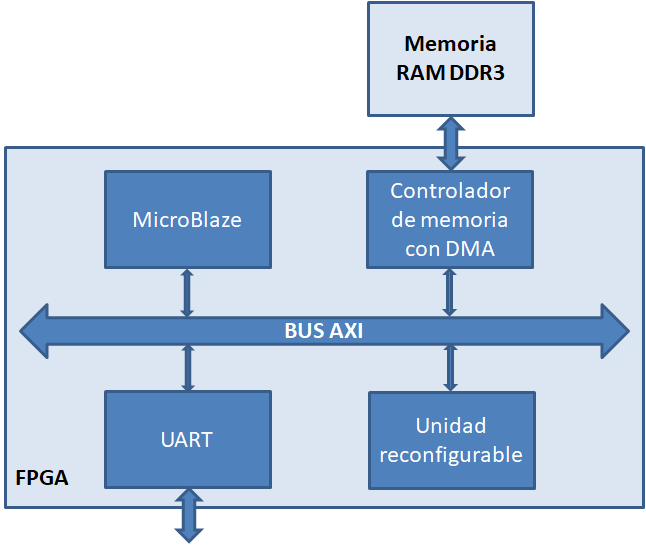
\includegraphics[width=0.7\textwidth]{images/plataforma_test.png}
  \caption{Plataforma de test para la placa VC709.}
  \label{fig:plataforma de test}
\end{figure}

El algoritmo completo en VHDL se ha implementado en una placa VC709 (ver Figura \ref{fig:VC709}), una placa reconfigurable con una sola Virtex-7 XC7VX690T, dos ranuras DDRM DDR3 que admiten hasta 4 GB cada una, un puerto RS232 y algunos componentes adicionales que no se han utilizado en nuestra implementación. La FPGA de Xilinx Virtex-7 XC7VX690T tiene una capacidad total de 693,120 celdas lógicas, 3,600 DSPs y 52,920 Kb de memoria.


Para llevar a cabo la validación del algoritmo en placa, se ha utilizado la plataforma de test que se muestra en la Figura \ref{fig:plataforma de test}. Como se puede observar, consta de un microprocesdor tipo MicroBlaze, un controlador de memoria, un puero serie y una unidad reconfigurable, todo ello interconectado mediante el bus AXI. Dentro de la unidad reconfigurable, se ubicaría el algoritmo a testear.

Por otro lado, para la implementación en OpenCL se ha hecho uso de la FPGA Intel Arria 10 GX 10AX115S2F45I2SGES (ver Tabla \ref{Arria10} para conocer los recursos disponibles y las particulariedades sobre el modelo de memoria en OpenCL). Este dispositivo se encuentra instalado en un servidor con un procesador Intel Xeon E5-1620 v3, con 4 cores físicos cada uno a una frecuencia de reloj de 3.5GHz y 64GB de memoria RAM DDR3. El sistema operativo empleado en este servidor es un CentOS Linux 7 y cuenta con la versión 17.1.0 del Intel FPGA SDK for OpenCL Offline Compiler.

\begin{table}[htb]
	\centering
	\begin{tabular}{|l|c|c|c|}
		\hline
		 & OpenCL & FPGA & Intel Arria 10 GX\\
		 \hline \hline
		 Memoria & Global & External &2GB DDR3\\ \hline 
		 & Constant &  Cache & 32KB DDR3\\ \hline 
		 & Local & Embedded & 67Mbits\\ \hline 
		 & Private & Registers & 67244Kbits \\ \hline
	\end{tabular}
	\caption{Modelo de memoria en OpenCL y recursos disponibles para la FPGA Intel Arria 10 GX.}
	\label{Arria10}
\end{table}

\section{Métricas}

\subsection{Calidad}
Antes de describir los resultados obtenidos, se describe primero la métrica utilizada para la comparación cuantitativa en los experimentos realizados. Con el fin de reducir el impacto de las fuentes de interferencia atmosférica en la evaluación realizada, se utiliza el ángulo espectral (AE) entre el endmember más similar detectado por la implementación propuesta y la firma espectral de referencia disponible en cada escena. El AE entre un píxel $X(i, j)$ seleccionado por el algoritmo ATGP-GS y una firma espectral de referencia $Si$ disponible a priori, puede calcularse simplemente como:

\begin{equation}\label{eq:ae}
AE[X(i,j), S_i] = cos^{-1} \frac{X(i,j) \cdot S_i}{|X(i,j)| \cdot |S_i|}
\end{equation}

es decir, el AE mide el ángulo formado por dos vectores n-dimensionales. Como resultado, valores bajos de AE significan una alta similitud espectral entre los vectores comparados. Esta medida de similitud espectral es independiente de la multiplicación de $X(i, j)$ y $Si$ por constantes y, en consecuencia, es independiente ante escalas multiplicativas desconocidas que puedan surgir debido a las diferencias en la iluminación y al ángulo de incidencia. Esto nos puede ayudar a compensar las diferentes condiciones de adquisición para un píxel en la imagen original y para una firma espectral recogida sobre el terreno (como es el caso de las firmas de referencia de la librería USGS utilizadas para la imagen AVIRIS Cuprite).

\subsection{Rendimiento}

Para medir el rendimiento se ha tenido en cuenta la aceleración del algoritmo en un lenguaje respecto al otro (ecuación~\ref{eq:metrica rendimiento}) y de esta manera realizar una comparativa entre ambos. Además, se ha identificado cuál es el tiempo límite (máximo) para que el procesamiento del desmezclado espectral de la imagen completa se pueda realizar en tiempo real \cite{tfg_miguel_carlos}, que es uno de los principales objetivos que se persigue en este trabajo.

\begin{equation}\label{eq:metrica rendimiento}
\text{Rendimiento} = \frac{\text{Tiempo OpenCL}}{\text{Tiempo VHDL}}
\end{equation}

%[SergioIni] Habría que darle una vuelta a este párrafo [SergioFin]

Pese a que las pruebas se realizarán sobre imágenes de un tamaño relativamente pequeño, es preciso destacar que si éstas se pueden procesar en tiempo real, las de mayor tamaño también se podrán procesar de esta forma. Esto se debe a que el aumento en el tiempo respecto al tamaño de la imagen es logarítmico, es decir, aumenta poco ante variaciones en el tamaño de las imágenes y/o en el número de endmembers a calcular.

Para medir el rendimiento, primero se analizará el rendimiento en cuanto a recursos empleados en cada implementación con la siguiente metodología: primero, se prestará atención a los recursos empleados (LUTs, LUTRAMs, BRAMs y DSPs) en la FPGA Virtex 7 XC7VX690T con el algorirmo en VHDL para imágenes de 188, 224 y 256 bandas, y se comparará con respecto a los máximos disponibles que ofrece el dispositivo; después, se realizará el mismo análisis pero respecto a la FPGA Intel Arria 10 GX y sus recursos (ALUTs, FFs, RAMs y DSPs), usando primero el algoritmo en OpenCL sin optimizaciones a modo de referencia y después con ellas.

Una vez determinado el rendimiento en cuanto a recursos utilizados, se procederá a evaluar el rendimiento en cuanto a tiempo. En primer lugar, se inferirá una fórmula que calcule el número de ciclos necesarios para analizar cualquier imagen a través del algoritmo en VHDL. Después se analizarán los tiempos de ejecución de las dos implementaciones con la imagen de Cuprite prestando atención para ello a la frecuencia de reloj. A continuación se establecerá una comparativa entre el tiempo teórico máximo alcanzable para un análisis a bordo y el tiempo real que tarda en ejecutarse el algoritmo en los lenguajes VHDL y OpenCL con la penalización de E/S. Finalmente con esta información se afirmará si se consigue viabilidad para un análisis en tiempo real o no.

\section{Resultados experimentales}

\subsection{Calidad}

\begin{table}[htbp]
	\centering
	\begin{tabular}{|l|c|c|}
		\hline
		Mineral en USGS & Implementación & Implementación \\
		 & OpenCL en FPGA & VHDL en FPGA \\ \hline \hline
		Alunita & 5.48$^{\circ}$ & 5.48$^{\circ}$ \\ \hline 
		Buddingtonita & 4.08$^{\circ}$ & 4.08$^{\circ}$ \\ \hline 
		Calcita & 5.87$^{\circ}$ & 5.87$^{\circ}$ \\ \hline 
		Kaolinita & 11.14$^{\circ}$ & 11.14$^{\circ}$ \\ \hline 
		Moscovita & 5.68$^{\circ}$ & 5.68$^{\circ}$ \\ \hline 
	\end{tabular}
	\caption{Ángulo espectral entre los endmembers extraídos en la escena AVIRIS Cuprite por las diferentes implementaciones de ATGP-GS y las firmas de referencia seleccionadas de la librería USGS.}
	\label{tabla2}
\end{table}

En la Tabla~\ref{tabla2} se muestra la calidad de los resultados experimentales tras la ejecución del algoritmo en OpenCL y en VHDL. Cabe señalar que sólo refleja la menor puntuación de AE de todos los endmembers extraídos con respecto a su firma de referencia en cada caso. Dado que se obtienen los mismos resultados, validamos que las dos implementaciones son correctas.

\subsection{Rendimiento}

En la Tabla~\ref{utilization virtex7} se pueden observar los resultados de ocupación en la FPGA Virtex-7 XC7VX690T, a partir de los cuales se puede afirmar que los recursos empleados en la implementación del algoritmo desarrollado en VHDL crecen linealmente con el número de bandas. Se observa que el recurso más utilizado son las LUTs y en el caso de un número de bandas elevado (256) apenas se alcanza un 86\% de su utilización.

\begin{table}[htb]\small
	\centering
	\begin{tabular}{|l|c|c|c|c|}
		\hline
		Recurso & LUT & LUTRAM & BRAM & DSP \\ \hline \hline
		Disponible & 433.200 & 174.200 & 1.470 & 3.600 \\ \hline 
		ATGP-GS (188 bandas)  & 271.912 (62,8\%) & 25.260 (14,5\%) & 475 (32,3\%) & 1.508 (41,9\%)  \\ \hline 
		ATGP-GS (224 bandas) & 311.496 (71,9\%) & 29.083 (16,7\%) & 555 (37,8\%) & 1.792 (49,8\%) \\ \hline 
		ATGP-GS (256 bandas) & 370.264 (85,5\%) & 34.397 (19,8\%) & 1.013 (68,9\%) & 2.118 (58,8\%)  \\ \hline
	\end{tabular}
	\caption{Resumen de la utilización de recursos en la Virtex--7 XC7VX690T.}
	\label{utilization virtex7}
\end{table}

\begin{table}[htb]\small
	\centering
	\begin{tabular}{|l|c|c|c|c|}
		\hline
		Recurso & ALUT & FF & RAM & DSP \\ \hline \hline
		Disponible & 707.600 & 1.415.440 & 2.531 & 1.518\\ \hline 
		ATGP-GS (sin optimizar) & 182.679 (25,8\%) & 354.680 (25,1\%) & 605 (23,9\%) & 24 (1,6\%)\\ \hline 
		ATGP-GS (188 bandas) & 210.515 (29,8\%) & 425.652 (30,1\%) & 941 (37,2\%) &  112 (7,4\%)\\ \hline
		ATGP-GS (224 bandas) & 217.325 (30,7\%) & 446.609 (31,6\%) & 1.043 (41,2\%) & 144 (9,5\%)\\ \hline
		ATGP-GS (256 bandas) & 226.709 (32,0\%) & 463.269 (32,7\%) & 1.144 (45,2\%) & 160 (10,5\%)\\ \hline
	\end{tabular}
	\caption{Resumen de la utilización de recursos en la Intel Arria 10 GX.}
	\label{utilization intel arria 10 gx}
\end{table}

En el caso de la implementación en OpenCL, los recursos necesarios crecen en la versión optimizada a medida que se varía el factor de la directiva \#\textit{pragma unroll num\_factor} para el desenrollado de bucles (ver Tabla~\ref{utilization intel arria 10 gx}), como consecuencia del tamaño de bandas espectrales. Para las imágenes Cuprite y sintética los factores óptimos han sido 12 y 16, respectivamente. Las demás optimizaciones no varían el porcentaje de recursos de la versión sin optimizar. En este caso se observa que el recurso más utilizado son las RAMs y apenas se alcanza un 46\% de su utilización.

El número de ciclos necesarios para la ejecución del algoritmo implementado en VHDL se puede calcular a partir de la siguiente fórmula:

\begin{gather}\label{eq:numero de ciclos algoritmo}
\text{núm.ciclos} = \underbrace{\text{núm.píxeles} + 16}_{\text{cálculo del primer target}} + \underbrace{\overbrace{47}^{\text{proyección}} + \text{ núm.píxeles} + 18\text{ }}_{\text{cálculo del segundo target}} + \underbrace{2 \cdot \text{núm.targets}}_{\text{peticiones y escrituras de targets}} + \nonumber\\\nonumber\\
\underbrace{\overbrace{103(\text{núm.targets} - 2) + \sum_{i=1}^{\text{núm.targets} - 2} (3i)}^{\text{proyecciones}} + (\text{núm.píxeles} + 18) \cdot (\text{núm.targets} - 2)}_{\text{cálculo del tercer target en adelante}}
\end{gather}

%donde p es el número de píxeles de la imagen y t es el número de targets a calcular.

en la que cabe destacar que el número de ciclos no depende del número de bandas sino únicamente del número de targets a calcular y del número de píxeles que contenga la imagen. Otro aspecto importante a tener en cuenta es que el ciclo de reloj se mantiene por encima de los 100 MHz y que se mantiene constante a pesar de que aumente el número de bandas espectrales. Teniendo esto en cuenta, para la imagen de Cuprite son necesarios 2.330.135 ciclos, por lo que el algoritmo se ejecutaría en 0,0233 segundos. Para la imagen sintética son necesarios 14.629.747 ciclos, por lo que se ejecutaría en 0,1463 segundos.

\begin{table}[htbp]
	\centering
	\begin{tabular}{|l|c|c|c|}
		\hline
		Imagen & Implementación OpenCL & Implementación VHDL & Implementación VHDL \\
		 &  & (plataforma test) & (máximo rendimiento) \\ \hline \hline
		Cuprite & 1,4874 seg & 0,3793 seg & 0,0233 seg \\ \hline 
		Sintética & 8,2089 seg & 1,8191 seg & 0,1463 seg \\ \hline 
	\end{tabular}
	\caption{Tiempo de procesamiento para la implementación del algoritmo ATDCA-GS desarrollado en VHDL y en OpenCL para FPGA.}
	\label{tabla5}
\end{table}

Observando la Tabla \ref{tabla5} se aprecia cómo los tiempos de ejecución en la plataforma de test para la implementación en VHDL son peores que los téoricos mínimos alcanzables para esta implementación. Esto se debe a que tal y como está desarrollada la plataforma de test, la E/S se convierte en el cuello de botella del sistema. Además, podemos observar cómo los tiempos de ejecución teóricos mínimos se incrementan sin tener en cuenta el número de bandas y sin embargo, para la implementación en la plataforma de test sí depende del número de banbas (se produce una mayor E/S). 

%[SergioIni] Estoy ahora mismo cerca del tiempo real para la imagen sintética...A ver si puedo bajarlo de alguna manera. Por lo demás este párrafo está OK [SergioFin]

Dado que el análisis en tiempo real de las imágenes se consigue cuando el tiempo de procesamiento es menor o igual que 1,986 segundos para la imagen de Cuprite o menor o igual que 7,903 segundos para la imagen sintética, se observa que, para la imagen Cuprite, sí se consigue un análisis eficiente con la implementacion tanto en VHDL como en OpenCL; para la imagen sintética, sí se consigue un análisis eficiente con la implementación en VHDL y, pese a que no ocurra lo mismo con la implementación en OpenCL, sí se alcanza un valor muy cercano al deseado. El tiempo teórico máximo para realizar un análisis a bordo de la imagen real y la sintética se obtiene tomando como referencia el sensor AVIRIS, que tarda 8,3 milisegundos en captar 512 píxeles con 224 bandas espectrales.

%Comentar que se consigue tiempo real con ambas implementaciones. Para Cuprite se considerará tiempo real si el tiempo de procesamiento es menor o igual a 1,986 segundos. Para la imagen sintética se considerará tiempo real si el tiempo de procesamiento es menor o  igual a 7,903 segundos. Estos dos tiempos salen si tomamos como referencia el sensor AVIRIS que tarda 8,3 milisegundos en captar 512 píxeles con 224 bandas espectrales